\documentclass[english,notitlepage,reprint,nofootinbib]{revtex4-1}  % defines the basic parameters of the document
% For preview: skriv i terminal: latexmk -pdf -pvc filnavn
% If you want a single-column, remove "reprint"

% Allows special characters (including æøå)
\usepackage[utf8]{inputenc}
% \usepackage[english]{babel}

%% Note that you may need to download some of these packages manually, it depends on your setup.
%% I recommend downloading TeXMaker, because it includes a large library of the most common packages.

\usepackage{physics,amssymb}  % mathematical symbols (physics imports amsmath)
\include{amsmath}
\usepackage{graphicx}         % include graphics such as plots
\usepackage{xcolor}           % set colors
\usepackage{hyperref}         % automagic cross-referencing
\usepackage{listings}         % display code
\usepackage{subfigure}        % imports a lot of cool and useful figure commands
\usepackage{float}
%\usepackage[section]{placeins}
\usepackage{algorithm}
\usepackage[noend]{algpseudocode}
\usepackage{subfigure}
\usepackage{tikz}
\usetikzlibrary{quantikz}
% defines the color of hyperref objects
% Blending two colors:  blue!80!black  =  80% blue and 20% black
\hypersetup{ % this is just my personal choice, feel free to change things
    colorlinks,
    linkcolor={red!50!black},
    citecolor={blue!50!black},
    urlcolor={blue!80!black}}


% ===========================================


\begin{document}
\raggedbottom

\title{Numerical simulation of the double-slit experiment \\using the 2+1 dimensional Schrödinger equation}  % self-explanatory
\author{Alessio Canclini, Filip von der Lippe} % self-explanatory
\date{\today}                             % self-explanatory
\noaffiliation                            % ignore this, but keep it.

%This is how we create an abstract section.
\begin{abstract}
    In this project, we investigate the behavior of a non-relativistic particle in two spatial dimensions. A simplified and dimensionless version of the time-dependent Schrödinger equation is used to recreate the famous double-slit experiment using computational methods. The equation is discretized using the Crank-Nicholson scheme and then implemented in C++. The initial wave function is given by a quantum mechanical Gaussian wave packet. To verify the code implementation we analyze the conservation of probability which theoretically should be fully conserved as $1.0$. The results show a maximum deviation of around $1.5 \times 10^{-14}$ without a barrier and  $1.4 \times 10^{-14}$ with a double-slit barrier. We deem this to be a sufficient conservation of probability resulting in acceptably accurate numerical simulation of the physical system. Color map plots of the 2D probability distribution for $t= 0.000, 0.001, 0.002$ display interference patterns after interacting with the double-slit barrier. These are studied more closely in color maps of the real and imaginary components of the wave packet where wave behavior is more obvious. The imaginary and real waves are slightly out of phase as expected. Finally, we study the interference pattern as a detection probability on a screen after the wave packet has passed through the slits. This is done for the typical double-slit case as well as a single- and triple-slit configuration. For the single-slit case we have an interference pattern with a single peak. The double- and triple-slit configurations results in interference patterns with five and seven probability peaks respectively.
\end{abstract}
\maketitle


% ===========================================
\section{Introduction}
%
Looking at the world around you there are an incredible variety of processes occurring. This can be the weather, how heat diffuses through your cooking utensils and burns you, or how light behaves and allows you to see it all. Most such physical processes are amazingly complex and depend on many variables. Partial differential equations (PDEs) allow us to model such processes.
These PDEs can be incredibly difficult and often impossible to solve analytically. An example readers might be familiar with are the famous Navier-Stokes equations, the solving of which would be rewarded with a million dollar prize \cite{millennium}. Thus, to simulate and at least approximate solutions to these equations we utilize the rapidly evolving tool of computational simulation by implementing a variety of finite difference schemes and letting a computer do the repetitive work.
We will use the Crank-Nicholson scheme to solve a possibly even more famous PDE, the time-dependent Schrödinger equation. The equation is simplified to our specific case where we simulate arguably the most famous experiment in physics; the double slit experiment. It was originally performed by Thomas Young around 1801 \cite{experiment} and has since been repeated in many ways to explore wave-particle duality.

Simple recreations of the double-slit experiment can be done at home, but an actual quantitative approach requires more specialized tools. By simulating it numerically one avoids investing in any specialized equipment as well as being able to change the experiments parameters with a literal click of a button.

The chosen Crank-Nicholson scheme is well suited for such a simulation as it is stable for all choices of temporal a and spatial step sizes and has reasonably small truncation errors of $\mathcal{O}(\Delta x^2)$, $\mathcal{O}(\Delta y^2)$ and $\mathcal{O}(\Delta t^2)$ \cite{compendium}.

First our numerical simulation is tested by studying how well it conserves probability. Once this is assessed and satisfactory we move on to analyzing the behavior in a double-slit case. Finally, a single- double- and triple-slit scenario are compared by studying the detection probability in each case on an imagined detector screen at $x=0.8$.

Section \ref{sec:methods} describes the theoretical background and gives an overview of the methods used for the simulations. The results are presented in section \ref{sec:results}. These and the methods are then discussed in section \ref{sec:discussion} followed by a summary and some concluding thoughts in section \ref{sec:conclusion}.

% ===========================================
\section{Methods}\label{sec:methods}
%
A GitHub repository containing code and more information on how to reproduce the results can be found following this link:
\url{https://github.com/Fslippe/FYS4150/tree/main/project5} \\ \\
To simulate the double-slit-in-a-box experiment we use the following theoretical framework. The time-dependent Schrödinger equation's general formulation is
\begin{equation}
    i \hbar \frac{d}{dt} | \Psi \rangle = \hat{H} | \Psi \rangle.
\end{equation}
Here $| \Psi \rangle$ is the quantum state and $\hat{H}$ is the Hamiltonian operator. For our purposes we consider a single, non-relativistic particle in two spatial dimensions. This allows $| \Psi \rangle$ to be expressed as $ \Psi (x,y,t)$, a complex-valued function. In this case the Schrödinger equation can be expressed as
\begin{align}
    i \hbar \frac{\partial}{\partial t} \Psi(x,y,t) = - \frac{\hbar^2}{2m} \left( \frac{\partial^2}{\partial x^2} + \frac{\partial}{\partial y^2}\right) \Psi(x,y,t) \\
    + V(x,y,t) \Psi (x,y,t). \nonumber
\end{align}
In the first term on the right hand side (RHS),
\begin{align*}
    - \frac{\hbar^2}{2m} \frac{\partial^2 \Psi}{\partial x^2} \quad\text{ and}\quad - \frac{\hbar^2}{2m} \frac{\partial^2 \Psi}{\partial x^2}
\end{align*}
express kinetic energy equivalent to $\frac{p^2}{2m}$ in classical physics. Here $m$ is the particle mass. Only the case of a time-independent potential $V = V(x,y)$ is considered. Working in this kind of position space the Born rule is
\begin{align}
    p(x,y;t) = |\Psi(x,y,t)|^2 = \Psi^{\ast} (x,y,t) \Psi(x,y,t).
\end{align}
Here $p(x,y;t)$ is the probability density of a particle being detected at a position $(x,y)$ at a time $t$. Continuing we assume that all dimensions have been scaled away. This leaves us with a dimensionless Schrödinger equation
\begin{equation}
    i \frac{\partial u}{\partial t} = - \frac{\partial^2 u}{\partial x^2} - \frac{\partial^2 u}{\partial y^2} + v(x,y)u. \label{eq:wave_eq}
\end{equation}
$v(x,y)$ is some potential and $u = u(x,y,t)$ our ``wave function'' which will hold a complex value ($u \in \mathbb{C}$). With this new notation the Born rule becomes
\begin{equation}
    p(x,y,;t) = |u(x,y,t)|^2 = u^{\ast} (x,y,t) u(x,y,t). \label{eq:born}
\end{equation}
$p(x,y,;t)$ is now a probability distribution.
Here we assume that the wave function $u$ has been properly normalized and $^*$ denotes the complex conjugate. For the simulations we will be working with $x \in [0,1]$, $y \in [0,1]$ and $t \in [0,T]$.


\subsection*{Notation}
To numerically describe our parameters we give $u(x,y,t)$, $v(x,y)$ and $p(x,y,t)$ a set of indices corresponding to a time and a two-dimensional position. This allows us to get the values of $u$, $v$ and $p$ for any chosen position and time. We define
\begin{align*}
    x \rightarrow x_i =ih, \quad y \rightarrow y_j =jh, \quad\text{and}\quad t \rightarrow  t_n =  n\Delta t.
\end{align*}
The values of $h$ and $\Delta t$ can be found in table \ref{tab:parameters}. From this we can describe the three-dimensional parameters for a position and time as
\begin{align*}
    u(x, y, t)  \rightarrow u_{ij}^n, \quad v(x, y) \rightarrow  v_{ij} \text{ }\text{ and }\text{ }  p(x, y, t) \rightarrow p_{ij}^n.
\end{align*}

\subsection*{Initial and boundary conditions}
Our potential $v_{ij}$ is defined to take the value $v_0$ at positions where we choose a wall to be and 0 otherwise. Depending on how many slits we chose when initializing the system, $v_{ij}$ is initialized differently with openings in the wall for any chosen aperture and distance between the slits. Any number of slits can be chosen as long as they will fit inside the wall length of 1, but in our case we will only look at none, one, two and three slits. We use the same parameters to describe the wall in all our experiments (except the no wall case) as shown in table \ref{tab:wall}.
\begin{table}[H]
    \begin{small}
        \caption{Parameters describing the setup of wall in our slit-experiments.}
        \label{tab:wall}
        \begin{center}
            \begin{tabular}{|l|l|}
                \hline
                \textbf{Parameter}                    & \textbf{Value} \\
                \hline
                Wall thickness in $x$ direction       & 0.02           \\
                \hline
                Wall position center in $x$ direction & 0.5            \\
                \hline
                Wall position center in $y$ direction & 0.5            \\
                \hline
                $y$ distance between slits            & 0.05           \\
                \hline
                slit aperture in $y$ direction        & 0.05           \\
                \hline
                potential in the wall ($v_0$)         & $10^{10}$      \\
                \hline
            \end{tabular}
        \end{center}
    \end{small}
\end{table}
We implement Dirichlet boundary conditions in the $xy$-plane as follows.
\begin{itemize}
    \item $u(x=0,y,t) = 0$
    \item $u(x=1,y,t) = 0$
    \item $u(x,y=0,t) = 0$
    \item $u(x,y=1,t) = 0$
\end{itemize}

The initial wave function $u_{ij}^0$ is given by the unnormalized quantum mechanical Gaussian wave packet
\begin{align}
    u(x,y,t = 0) = e^{-\frac{(x-x_c)^2}{2 \sigma_x^2} -\frac{(y-y_c)^2}{2 \sigma_y^2}+ ip_x (x-x_c)+ ip_y (y-y_c)}. \label{eq:wave_func}
\end{align}
$x_c$ and $y_c$ are the coordinates of the center of the initial wave packet. The width of the initial wave packet in the $x$ and $y$ direction are $\sigma_x$ and $\sigma_y$ and the wave packet momenta are $p_x$ and $p_y$. $u_{ij}^n$ for all $i$ and $j$ are values in a matrix $U^n$ that denotes the 2D state of $u$ at time step $n$. The initial state is normalized such that
\begin{equation}
    \sum_{i,j} u_{ij}^{0*} u_{ij}^0 = 1,
\end{equation}
where $^*$ again denotes the complex conjugate.

For all our simulations we will use the same values of some initial parameters as seen in table \ref{tab:parameters}.
\begin{table}[H]
    \begin{small}
        \caption{Parameters used to describe the initial wave packet and the step sizes.}
        \label{tab:parameters}
        \begin{center}
            \begin{tabular}{|l|l|}
                \hline
                \textbf{Parameter}                                  & \textbf{Value}      \\
                \hline
                $x$-center of initial wave packet ($x_c$)           & 0.25                \\
                \hline
                $y$-center of initial wave packet ($y_c$)           & 0.5                 \\
                \hline

                Momentum in $x$-direction ($p_x$)                   & 200                 \\
                \hline
                Momentum in $y$-direction ($p_y$)                   & 0                   \\
                \hline
                Width of initial wave in $x$-direction ($\sigma_x$) & 0.05                \\
                \hline
                Width of initial wave in $y$-direction ($\sigma_y$) & 0.05, 0.1 or 0.2    \\
                \hline
                Time step size ($\Delta t$)                         & $2.5\times 10^{-5}$ \\
                \hline
                Position step size ($h$)                            & $0.005$             \\
                \hline
            \end{tabular}
        \end{center}
    \end{small}
\end{table}

\subsection*{The Crank-Nicholson scheme}
Crank-Nicholson (CN) is an unconditionally stable numerical scheme with truncation errors $\mathcal{O}(\Delta x^2)$, $\mathcal{O}(\Delta y^2)$ and $\mathcal{O}(\Delta t^2)$ \cite{compendium}. In our case we use the same step size for $x$ and $y$ such that $\Delta x = \Delta y = h$. Using the CN scheme, eq. \ref{eq:wave_eq} is discretized as
\begin{align} \label{eq:CN}
     & u_{ij}^{n+1} - r \left[ u_{i+1,j}^{n+1}- 2 u_{ij}^{n+1} + u_{i-1,j}^{n+1} \right] \nonumber \\
     & - r \left[ u_{i,j+1}^{n+1}- 2 u_{ij}^{n+1} + u_{i,j-1}^{n+1} \right]
    + \frac{i \Delta t}{2} v_{ij} u_{ij}^{n+1}                                                     \\
     & = u_{ij}^n
    + r \left[ u_{i+1,j}^{n}- 2 u_{ij}^{n} + u_{i-1,j}^{n} \right] \nonumber                       \\
     & + r \left[ u_{i,j+1}^{n}- 2 u_{ij}^{n} + u_{i,j-1}^{n} \right]
    - \frac{i \Delta t}{2} v_{ij} u_{ij}^{n}. \nonumber
\end{align}
Here $r \equiv \frac{i \Delta t}{2h^2}$. $i$ indexes are not to be confused with the imaginary unit $i$. A more comprehensive analytical derivation can be found in appendix \ref{appendix:analytic}. Considering the case with our specific boundary conditions, this can be expressed as the matrix equation
\begin{equation}
    A \vec{u}^{\text{ }n+1} = B \vec{u}^{\text{ }n}. \label{eq:matrix}
\end{equation}
To solve eq. \ref{eq:matrix} we choose to use a solver from the armadillo library specifically for sparse systems of linear equations. Since $A$ and $B$ are sparse matrices, this lowers the computational cost. The solver performs an LU decomposition with partial pivoting and triangular system solves through forward and back substitution \cite{superlu_ug99}.

A slight complication when solving eq. \ref{eq:matrix} is that we want to calculate 2D $U^n$ matrices for each time step $n$, but the CN matrix equation requires these values to be in vector form $\vec{u}$. In the code this is resolved by implementing an index translation function to facilitate changing between matrix and vector form.
\begin{align*}
    k =(i - 1) + (M - 2) (j - 1)
\end{align*}
translates two $(i,j)$ matrix indices to a single vector index $k$.
% ===========================================
\section{Results}\label{sec:results}
%
Figure \ref{fig:no_slit_p_diff} and \ref{fig:double_slit_p_diff} show how much the total probability deviation from 1.0 as a function of time. Figure \ref{fig:no_slit_p_diff} shows the results without any slits in the wall. The results in  figure \ref{fig:double_slit_p_diff} are for a double slit case and a slightly broader initial wave packet in the $y$ direction.
% prob 7 plots
\begin{figure}[H]
    \centering
    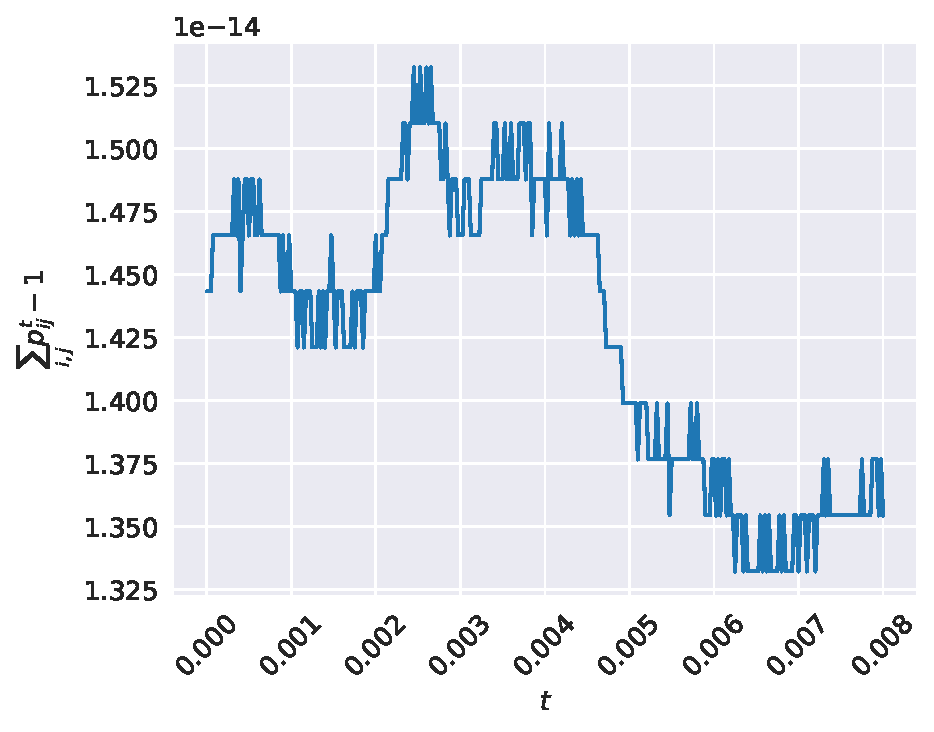
\includegraphics[width=.5\textwidth]{../figures/no_slit_p_diff.pdf}
    \caption{Deviation of the total probability from 1.0 as a function of time without a double-slit barrier. \\Simulation settings: $h = 0.005, \Delta t = 2.5 \times 10^{-5}, \\T = 0.008, x_c = 0.25, \sigma_x = 0.05, p_x = 200, y_c = 0.5, \\\sigma_y = 0.05, p_y = 0, v_0 = 0$.}
    \label{fig:no_slit_p_diff}
\end{figure}

\begin{figure}[H]
    \centering
    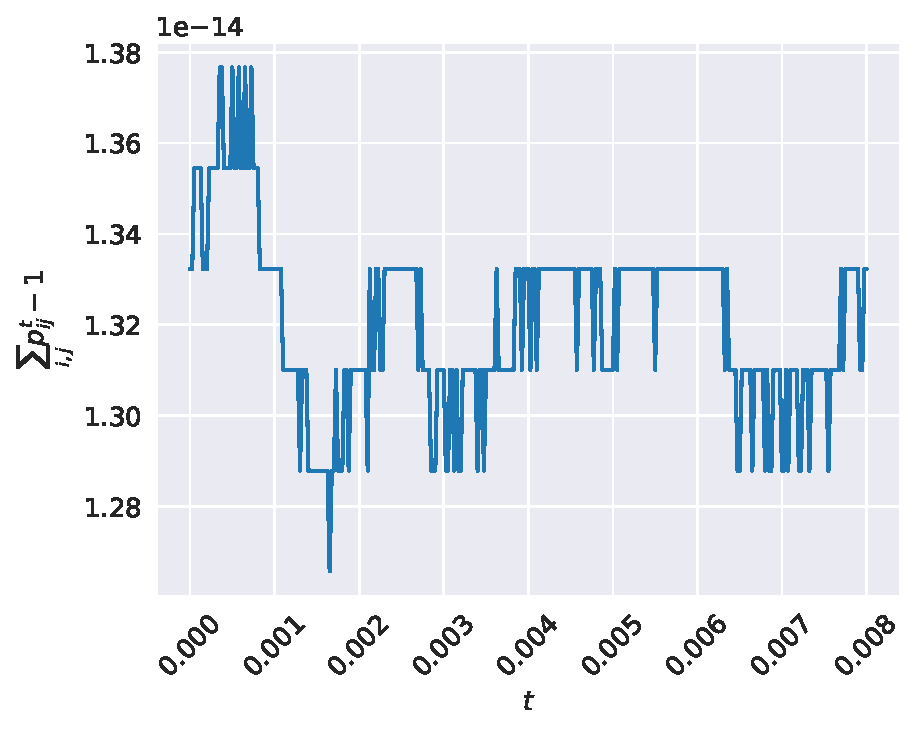
\includegraphics[width=.5\textwidth]{../figures/double_slit_p_diff.pdf}
    \caption{Deviation of the total probability from 1.0 as a function of time with two slits. \\Simulation settings: $h = 0.005, \Delta t = 2.5 \times 10^{-5}, \\T = 0.008, x_c = 0.25, \sigma_x = 0.05, p_x = 200, y_c = 0.5, \\\sigma_y = 0.1, p_y = 0, v_0 = 1 \times 10^{10}$.}
    \label{fig:double_slit_p_diff}
\end{figure}
In both cases the probability deviation fluctuates, but is tiny. With a maximal deviation of about $1.5 \times 10^{-14}$ the results show a good conservation of probability over the simulated time interval of $t \in [0,0.008]$. This shows that the code woks as desired.

Having checked the general functionality of the code we move on to plotting the 2D probability distribution $p$ for $t=0.000, 0.001, 0.002$ in figure \ref{fig:double_slit_0.000}, \ref{fig:double_slit_0.001} and \ref{fig:double_slit_0.002} respectively. In all following plots the vertical black line centered along $x$ is the double-slit barrier.

%prob 8 color map plots
% t=0
\begin{figure}[H]
    \centering
    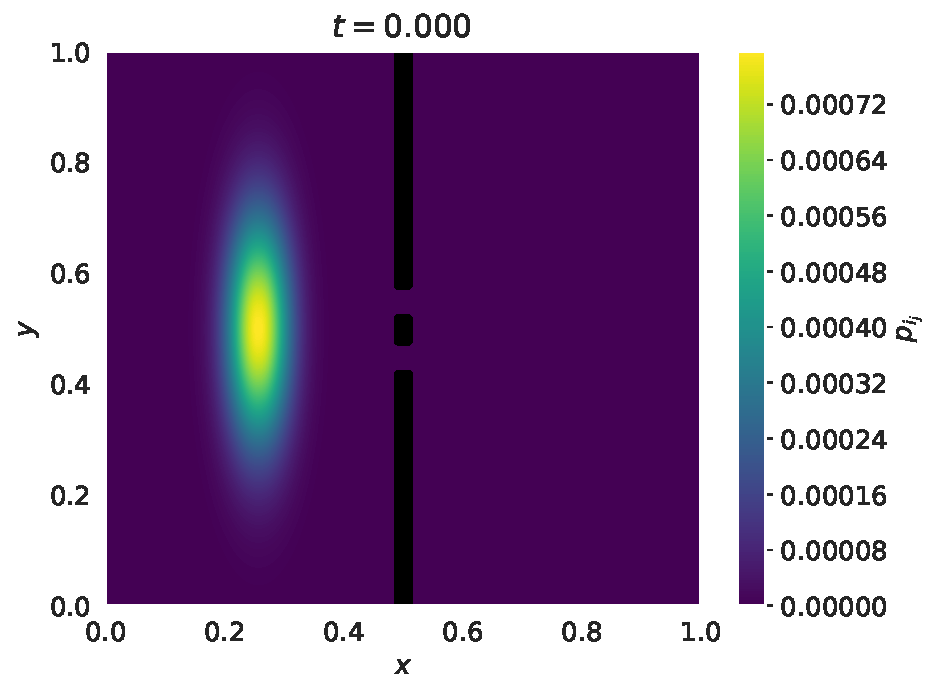
\includegraphics[width=.5\textwidth]{../figures/double_slit_0.000.pdf}
    \caption{Color map of the 2D probability distribution at \\$t = 0.000$. \\Simulation settings: $h = 0.005, \Delta t = 2.5 \times 10^{-5}, \\T = 0.00, x_c = 0.25, \sigma_x = 0.05, p_x = 200, y_c = 0.5, \\\sigma_y = 0.20, p_y = 0, v_0 = 1 \times 10^{10}$.}
    \label{fig:double_slit_0.000}
\end{figure}
% t=0.001
\begin{figure}[H]
    \centering
    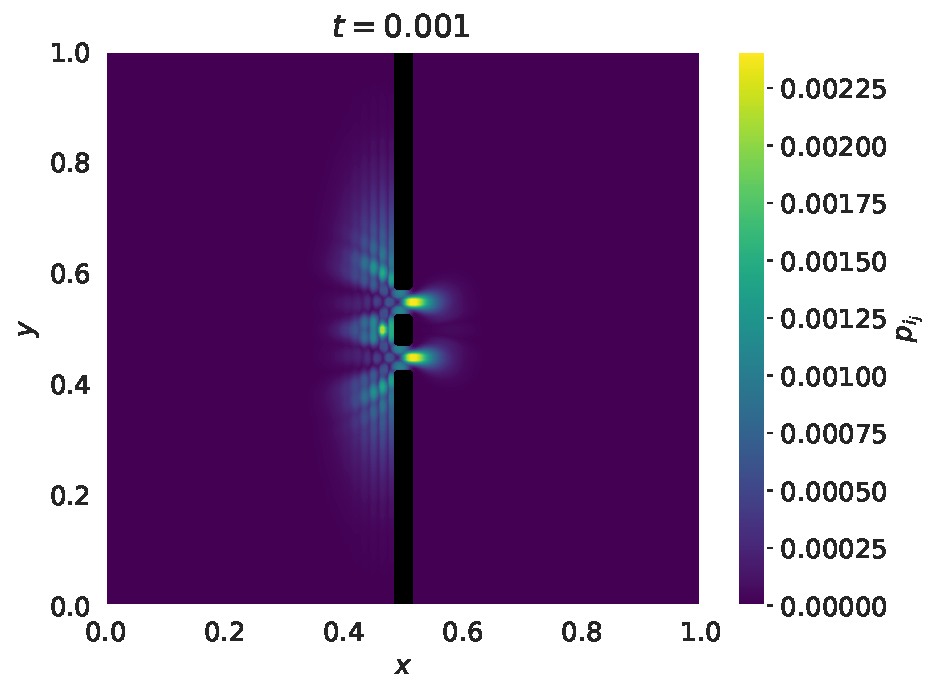
\includegraphics[width=.5\textwidth]{../figures/double_slit_0.001.pdf}
    \caption{Color map of the 2D probability distribution at \\$t = 0.001$. \\Simulation settings: $h = 0.005, \Delta t = 2.5 \times 10^{-5}, \\T = 0.00, x_c = 0.25, \sigma_x = 0.05, p_x = 200, y_c = 0.5, \\\sigma_y = 0.20, p_y = 0, v_0 = 1 \times 10^{10}$.}
    \label{fig:double_slit_0.001}
\end{figure}
% t=0.002
\begin{figure}[H]
    \centering
    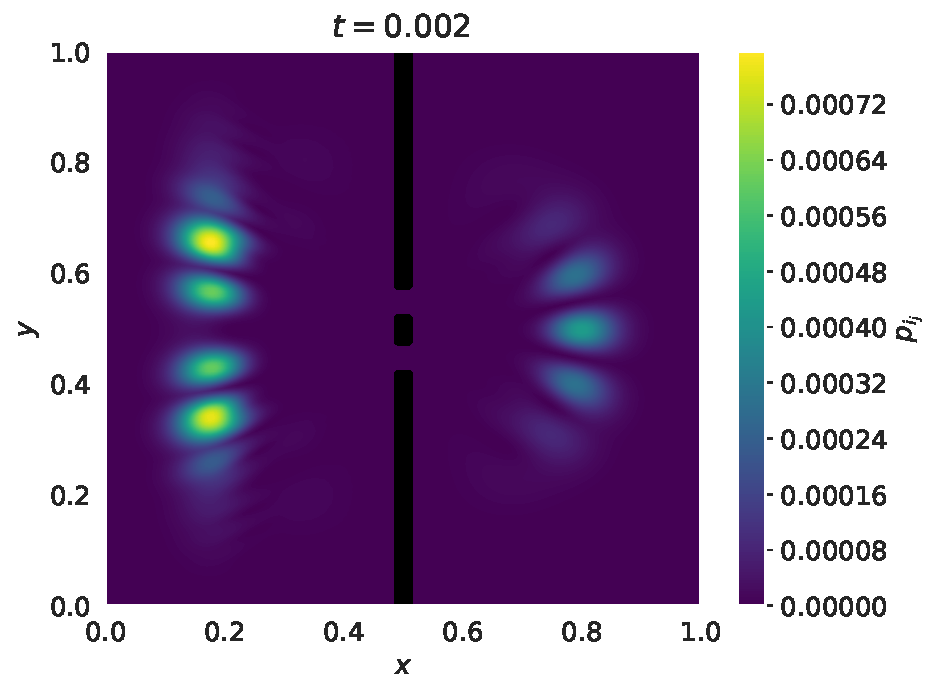
\includegraphics[width=.5\textwidth]{../figures/double_slit_0.002.pdf}
    \caption{Color map of the 2D probability distribution at \\$t = 0.002$. \\Simulation settings: $h = 0.005, \Delta t = 2.5 \times 10^{-5}, \\T = 0.00, x_c = 0.25, \sigma_x = 0.05, p_x = 200, y_c = 0.5, \\\sigma_y = 0.20, p_y = 0, v_0 = 1 \times 10^{10}$.}
    \label{fig:double_slit_0.002}
\end{figure}
Noticeably in figure \ref{fig:double_slit_0.001} one can see that the interaction with the  wall and slits happens just before $t=0.001$. Figure \ref{fig:double_slit_0.002} shows that parts of the probability distribution ``pass through'' the slits, whilst the rest is ``reflected'' back in the other direction. An animation of the full sequence can be found following this link: \url{https://github.com/Fslippe/FYS4150/blob/main/project5/figures/animation.gif}. Initially at $t=0.000$ in figure \ref{fig:double_slit_0.000} the probability density shows one cohesive area of higher probability. After interacting with the slits there are several, separate non-zero probability areas as seen in figure \ref{fig:double_slit_0.002}.

To investigate the wave function $u$, figures \ref{fig:double_slit_real_0.000}, \ref{fig:double_slit_real_0.001} and \ref{fig:double_slit_real_0.002} show $\Re(u_{ij})$ for $t=0.000, 0.001, 0.002$.
%only Re 
% t=0
\begin{figure}[H]
    \centering
    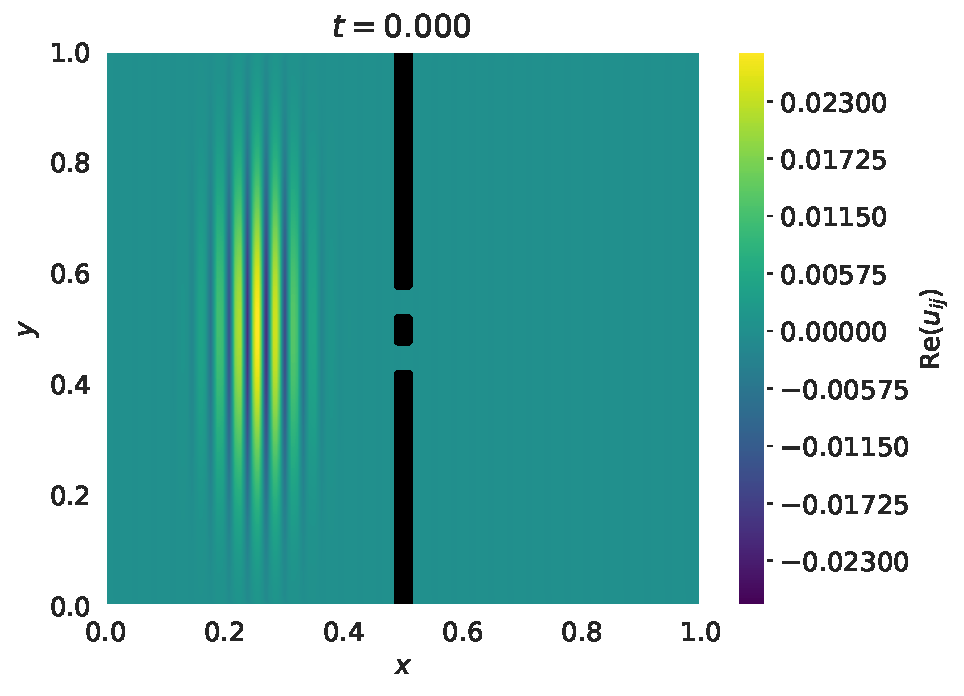
\includegraphics[width=.5\textwidth]{../figures/double_slit_real_0.000.pdf}
    \caption{Color map of $\Re (u_{ij})$ at $t = 0.000$. \\Simulation settings: $h = 0.005, \Delta t = 2.5 \times 10^{-5}, \\T = 0.00, x_c = 0.25, \sigma_x = 0.05, p_x = 200, y_c = 0.5, \\\sigma_y = 0.20, p_y = 0, v_0 = 1 \times 10^{10}$.}
    \label{fig:double_slit_real_0.000}
\end{figure}
% t=0.001
\begin{figure}[H]
    \centering
    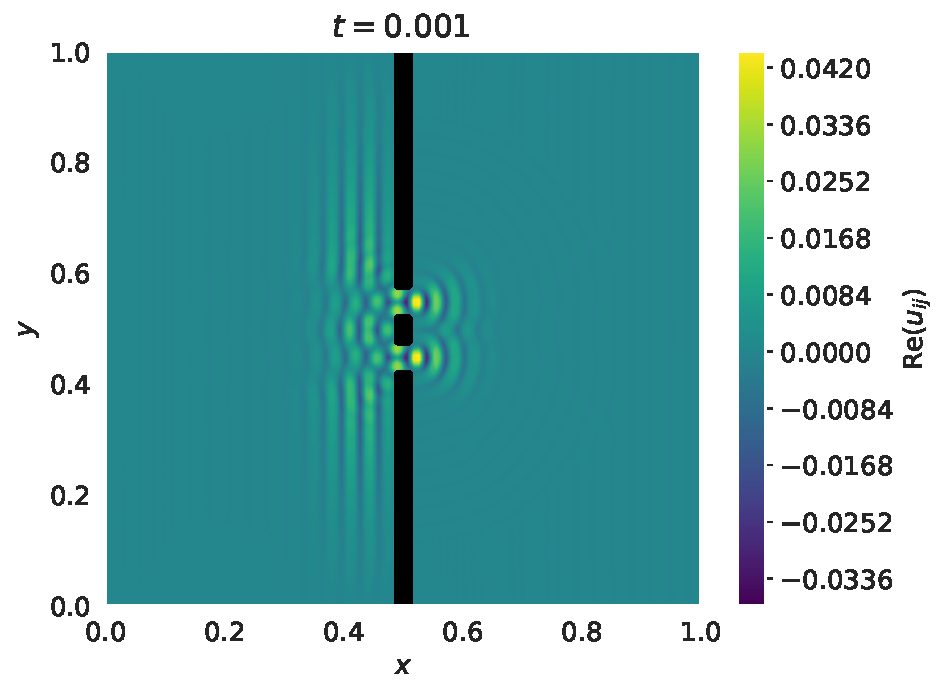
\includegraphics[width=.5\textwidth]{../figures/double_slit_real_0.001.pdf}
    \caption{Color map of $\Re (u_{ij})$ at $t = 0.001$.  \\Simulation settings: $h = 0.005, \Delta t = 2.5 \times 10^{-5}, \\T = 0.00, x_c = 0.25, \sigma_x = 0.05, p_x = 200, y_c = 0.5, \\\sigma_y = 0.20, p_y = 0, v_0 = 1 \times 10^{10}$.}
    \label{fig:double_slit_real_0.001}
\end{figure}
% t=0.002
\begin{figure}[H]
    \centering
    \includegraphics[width=.5\textwidth]{../figures/double_slit_real_0.002.pdf}
    \caption{Color map of $\Re (u_{ij})$ at $t = 0.002$.  \\Simulation settings: $h = 0.005, \Delta t = 2.5 \times 10^{-5}, \\T = 0.00, x_c = 0.25, \sigma_x = 0.05, p_x = 200, y_c = 0.5, \\\sigma_y = 0.20, p_y = 0, v_0 = 1 \times 10^{10}$.}
    \label{fig:double_slit_real_0.002}
\end{figure}

%only Im
% t=0
\begin{figure}[H]
    \centering
    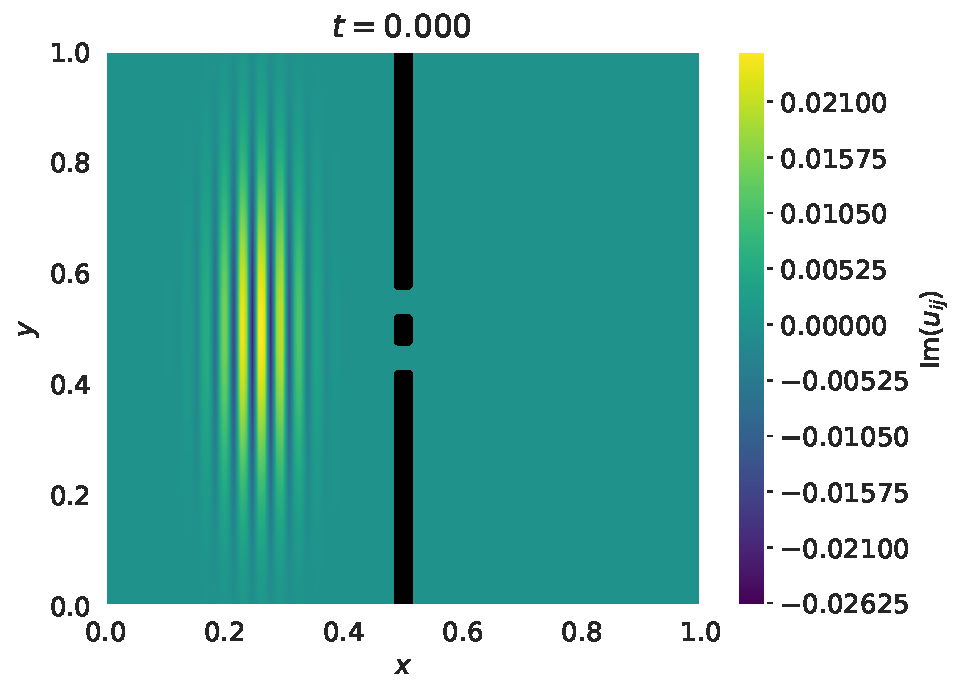
\includegraphics[width=.5\textwidth]{../figures/double_slit_imag_0.000.pdf}
    \caption{Color map of $\Im (u_{ij})$ at $t = 0.000$. \\Simulation settings: $h = 0.005, \Delta t = 2.5 \times 10^{-5}, \\T = 0.00, x_c = 0.25, \sigma_x = 0.05, p_x = 200, y_c = 0.5, \\\sigma_y = 0.20, p_y = 0, v_0 = 1 \times 10^{10}$.}
    \label{fig:double_slit_imag_0.000}
\end{figure}
A full animation of the $\Re(u_{ij})$ behaviour can be found following this link: \url{https://github.com/Fslippe/FYS4150/blob/main/project5/figures/animation_real.gif}.
Figures \ref{fig:double_slit_imag_0.000}, \ref{fig:double_slit_imag_0.001} and \ref{fig:double_slit_imag_0.002} show $\Im(u_{ij})$ for $t=0.000, 0.001, 0.002$.
% t=0.001
\begin{figure}[H]
    \centering
    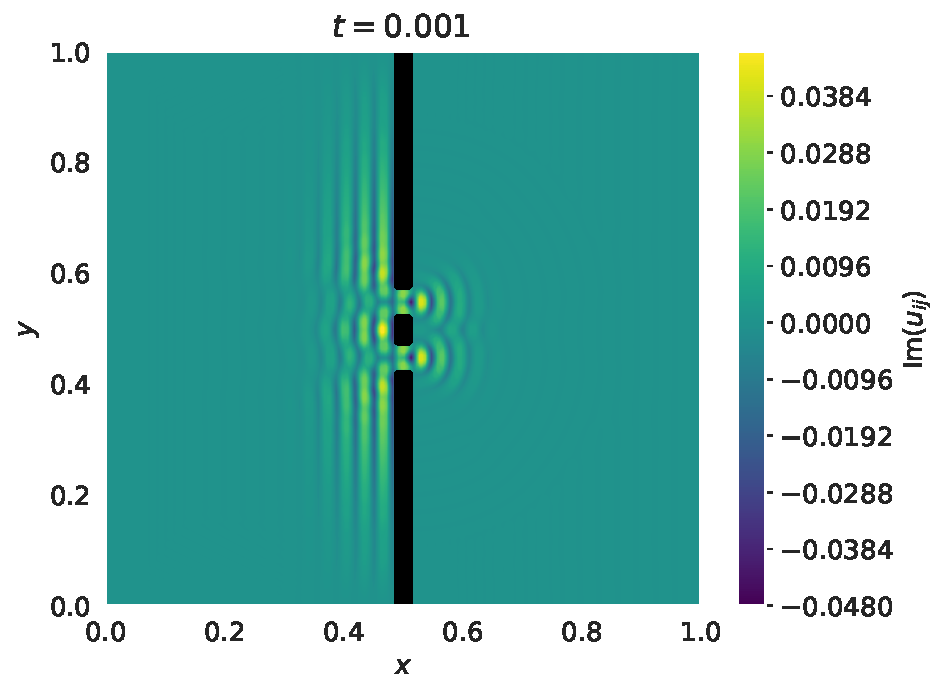
\includegraphics[width=.5\textwidth]{../figures/double_slit_imag_0.001.pdf}
    \caption{Color map of $\Im (u_{ij})$ at $t = 0.001$. \\Simulation settings: $h = 0.005, \Delta t = 2.5 \times 10^{-5}, \\T = 0.00, x_c = 0.25, \sigma_x = 0.05, p_x = 200, y_c = 0.5, \\\sigma_y = 0.20, p_y = 0, v_0 = 1 \times 10^{10}$.}
    \label{fig:double_slit_imag_0.001}
\end{figure}
% t=0.002
\begin{figure}[H]
    \centering
    \includegraphics[width=.5\textwidth]{../figures/double_slit_imag_0.002.pdf}
    \caption{Color map of $\Im (u_{ij})$ at $t = 0.002$. \\Simulation settings: $h = 0.005, \Delta t = 2.5 \times 10^{-5}, \\T = 0.00, x_c = 0.25, \sigma_x = 0.05, p_x = 200, y_c = 0.5, \\\sigma_y = 0.20, p_y = 0, v_0 = 1 \times 10^{10}$.}
    \label{fig:double_slit_imag_0.002}
\end{figure}
Figures \ref{fig:double_slit_real_0.000}, \ref{fig:double_slit_real_0.001}, \ref{fig:double_slit_real_0.002}, \ref{fig:double_slit_imag_0.000}, \ref{fig:double_slit_imag_0.001} and \ref{fig:double_slit_imag_0.002} all show wave-like characteristics with lighter colored peaks and darker thoughts. The imaginary and real components display very similar behavior, but for slightly different values. The initial wave packet in figure \ref{fig:double_slit_real_0.000} and \ref{fig:double_slit_imag_0.000} has several peaks along the $x$-axis, but only one along the $y$-axis. When the wave interacts with the slits in figure \ref{fig:double_slit_real_0.001} and \ref{fig:double_slit_imag_0.001} we see two new and separate waves originate. One from each slit. Whereas the initial wave was moving in a positive $y$ direction, these new waves propagate in all radial directions where not obstructed by the wall. Focusing on the right side of the wall in figure \ref{fig:double_slit_real_0.002} and \ref{fig:double_slit_imag_0.002} we observe lines of lower amplitudes interrupting the somewhat circular wave pattern.

% prob 9 detector screen
To replicate the particle detector screen in a physical slit experiment figure \ref{fig:prob_y_normalized_0.002_x_0.8}, \ref{fig:single_prob_y_normalized_0.002_x_0.8} and \ref{fig:tripple_prob_y_normalized_0.002_x_0.8} show the detection probability along a screen spanning all of $y$ at $x = 0.8$. As we expect to detect every particle at some point along $y$, the one dimensional probability function has been normalized such that it sums to $1.0$.
% double slit
\begin{figure}[H]
    \centering
    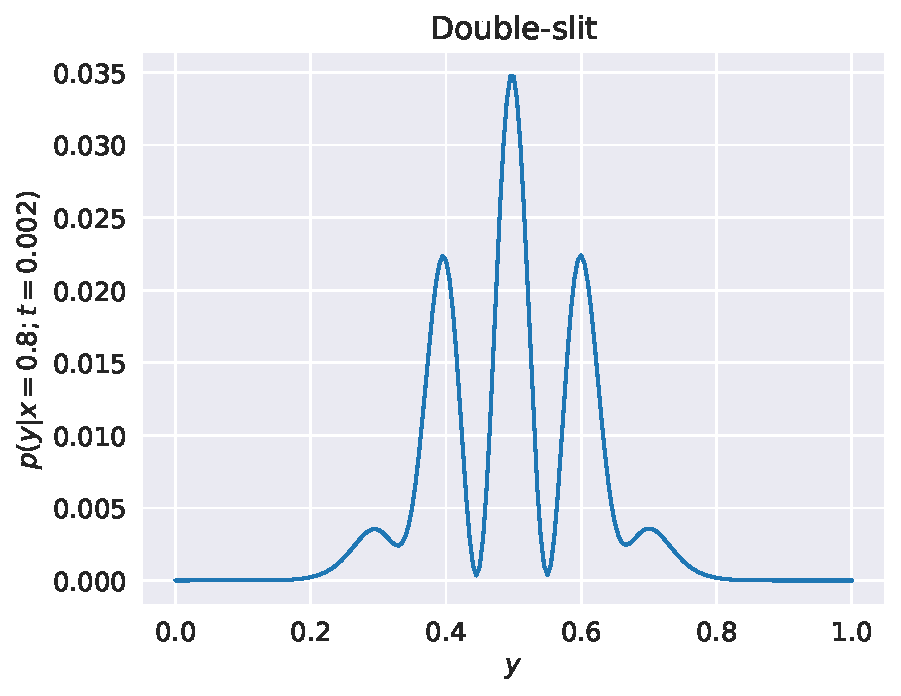
\includegraphics[width=.5\textwidth]{../figures/prob_y_normalized_0.002_x_0.8.pdf}
    \caption{ Detection probability along a screen at $x =0.8$ for a double-slit scenario. \\Simulation settings: $h = 0.005, \Delta t = 2.5 \times 10^{-5}, \\T = 0.00, x_c = 0.25, \sigma_x = 0.05, p_x = 200, y_c = 0.5, \\\sigma_y = 0.20, p_y = 0, v_0 = 1 \times 10^{10}$.}
    \label{fig:prob_y_normalized_0.002_x_0.8}
\end{figure}
%single slit
\begin{figure}[H]
    \centering
    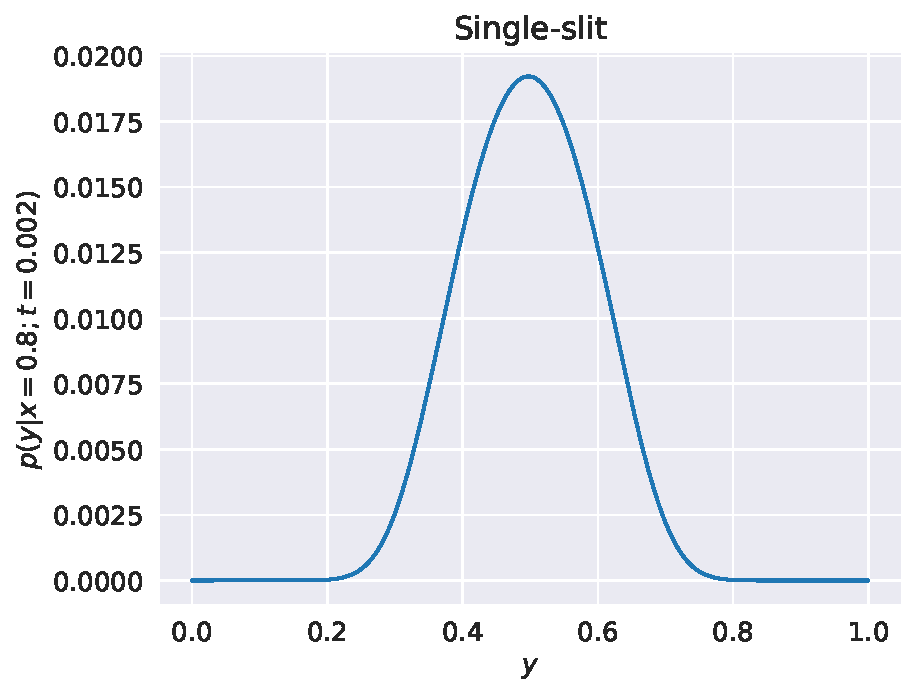
\includegraphics[width=.5\textwidth]{../figures/single_prob_y_normalized_0.002_x_0.8.pdf}
    \caption{Detection probability along a screen at $x =0.8$ for a single-slit scenario. \\Simulation settings: $h = 0.005, \Delta t = 2.5 \times 10^{-5}, \\T = 0.00, x_c = 0.25, \sigma_x = 0.05, p_x = 200, y_c = 0.5, \\\sigma_y = 0.20, p_y = 0, v_0 = 1 \times 10^{10}$.}
    \label{fig:single_prob_y_normalized_0.002_x_0.8}
\end{figure}
% triple slit
\begin{figure}[H]
    \centering
    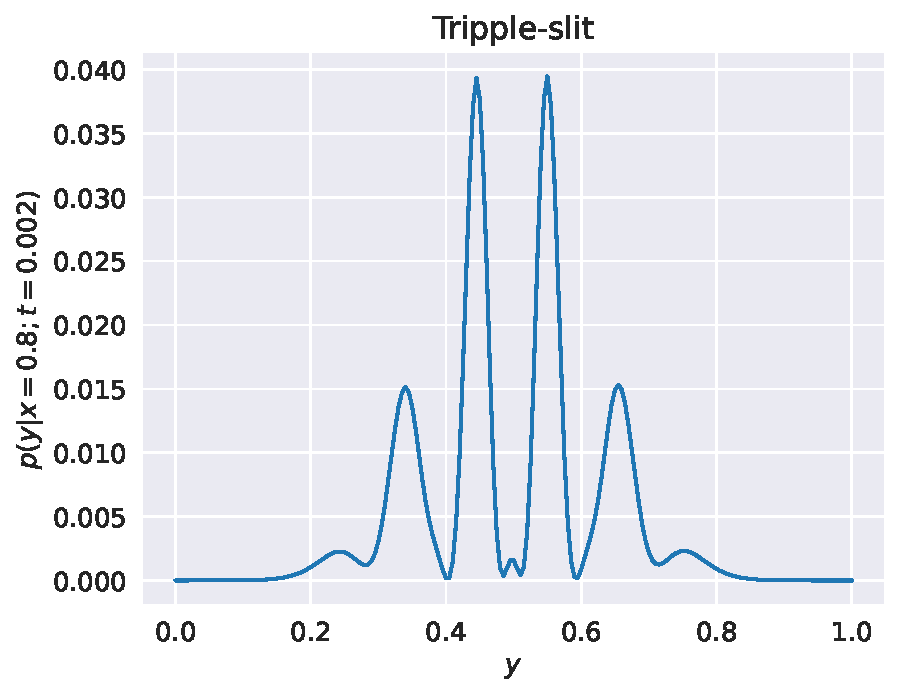
\includegraphics[width=.5\textwidth]{../figures/tripple_prob_y_normalized_0.002_x_0.8.pdf}
    \caption{Detection probability along a screen at $x =0.8$ for a triple-slit scenario. \\Simulation settings: $h = 0.005, \Delta t = 2.5 \times 10^{-5}, \\T = 0.00, x_c = 0.25, \sigma_x = 0.05, p_x = 200, y_c = 0.5, \\\sigma_y = 0.20, p_y = 0, v_0 = 1 \times 10^{10}$.}
    \label{fig:tripple_prob_y_normalized_0.002_x_0.8}
\end{figure}
Comparing figure \ref{fig:prob_y_normalized_0.002_x_0.8}, \ref{fig:single_prob_y_normalized_0.002_x_0.8} and \ref{fig:tripple_prob_y_normalized_0.002_x_0.8} we see that different slit configurations result in different detection probabilities. For the case of one slit in figure \ref{fig:single_prob_y_normalized_0.002_x_0.8} there is only one peak. In the case of two and three slits on the other hand we observe five and seven peaks respectively.

% ===========================================
\section{Discussion}\label{sec:discussion}
% Conservation of probability
We begin by verifying the functionality of our numerical 2+1 dimensional Schrödinger equation simulation. This is done by studying the conservation of probability which in theory should be fully conserved. Figure \ref{fig:no_slit_p_diff} and \ref{fig:double_slit_p_diff} both show extremely low deviation values with a maximum around $1.525 \times 10^{-14}$ and $1.38 \times 10^{-14}$ for cases without and with a double-slit barrier respectively. Such small deviations could be attributed to the computer's floating point number precision, leading to round off errors.  This can also potentially be affected by the chosen method of solving eq. \ref{eq:matrix} which explains how the deviation changes over time. A more accurate analysis would require further research comparing different methods for solving the matrix equation and a variety of finite differencing shcemes.
Since the deviation stays at the same order of magnitude over the time period, it is clear that the time stepping process is not the main contributor to the deviation. This indicates that the normalization at $t=0$ is what mainly gives us a deviation from 0. When comparing the deviation plots to what we see in figure \ref{fig:double_slit_0.000}, \ref{fig:double_slit_0.001} and \ref{fig:double_slit_0.002} and the animation found at: \url{https://github.com/Fslippe/FYS4150/blob/main/project5/figures/animation.gif}, it is clear that the collision with the walls and the slits has an influence on the deviation. This can be explained by the fast accelerations and spreading of the wave packet in these areas, changing the values our solver has to work with. For no slits we see such changes as expected around $t=$ 0.002, 0.004 and 0.006 corresponding to when the wave packet may hit the boundaries. In the double slit case we see as expected an additional abrupt change at $t=0.001$ which corresponds to the first interaction with the slits. Such a change only with a smaller deviation can also be seen for no slits in figure \ref{fig:no_slit_p_diff} which cannot be explained by a sudden acceleration change. This leads to an uncertainty around the reason for these changes, also in the double slit case in figure \ref{fig:double_slit_p_diff}. Since the deviation from the total probability of $1.0$ for $t \in [0,0.008]$ is close to zero we can in total consider the probability conserved. Thus, the code is suitable for further simulations.

%Color maps of probability + animation

%Color maps og Im and Re
Now consider the wave function in eq. \ref{eq:wave_func}. Using Euler's formula $e^{ix} = \cos(x) + i \sin(x)$ it can be expressed as
\begin{equation}
    u(x,y,t = 0) = A \cos(\phi) + A i \sin(\phi),
\end{equation}
where we have
\begin{align}
    \phi & = p_x (x-x_c)+ p_y (y-y_c) \text{  and} \\ A &= e^{-\frac{(x-x_c)^2}{2 \sigma_x^2} -\frac{(y-y_c)^2}{2 \sigma_y^2}}.
\end{align}
We see that the real term is a cosine function and the imaginary term is a sine function. This explains what seems to be a slightly different phase for $\Re(u_{ij})$ in figure \ref{fig:double_slit_real_0.000} and $\Im(u_{ij})$ in figure \ref{fig:double_slit_imag_0.000} as there is a $\frac{\pi}{2}$rad phase difference between the two functions. Individually these two values don't give enough information to describe the system, but applying the born rule in eq. \ref{eq:born} when working in a discretized space gives us a certain probability distribution. Noticeably the probability distribution results in figure \ref{fig:double_slit_0.000}, \ref{fig:double_slit_0.001} and \ref{fig:double_slit_0.002} show very similar patterns to figure \ref{fig:double_slit_real_0.000}, \ref{fig:double_slit_real_0.001}, \ref{fig:double_slit_real_0.002}, \ref{fig:double_slit_imag_0.000}, \ref{fig:double_slit_imag_0.001} and \ref{fig:double_slit_imag_0.002} when comparing for the same values of $t$. To describe the observed phenomena we will take a closer look at the $\Re(u_{ij})$ results and use these to explain the actual probability distribution. When the initial wave hits the double-slit barrier in figure \ref{fig:double_slit_real_0.001} it gives rise to a new wave pattern. This looks comparable to a pattern that would originate when dropping two stones into water. The waves propagate outwards from each slit (much like they would form each stone in water). In this case they do this in the direction of travel, but now with a circular pattern. The two circular patterns then start to collide resulting in the pattern observed at $t = 0.002$ in figure \ref{fig:double_slit_real_0.002}. Here we observe interference. Peaks of waves colliding with other peaks and troughs colliding with troughs result in constructive interference, an increase in amplitude. The most interesting behavior is where peaks and troughs of two waves meet, these cancel each other out resulting in destructive interference and thus the wave amplitude diminishing. This destructive interference is what causes the radial lower value lines in figure \ref{fig:double_slit_real_0.002} and equivalently the radial lower probability regions in figure \ref{fig:double_slit_0.002}.


Studying the interference plots in figure \ref{fig:prob_y_normalized_0.002_x_0.8}, \ref{fig:single_prob_y_normalized_0.002_x_0.8} and \ref{fig:tripple_prob_y_normalized_0.002_x_0.8}
we see a different number of probability peaks. For only one slit we see what looks like a Gaussian probability distribution with the most probable position being the same as the center of the slit. This makes sense form how the wave packet is defined with its most probable initial state being $y=0.5$ meaning that a movement in x-direction without any interference would conserve the most probable position. For both the double and triple-slit experiments we see what looks like a Gaussian distribution only with dips in the probability for some values. This matches the characteristic interference pattern that one expects when performing a double-slit (and in this case triple-slit) experiment. As described earlier this happens because of destructive interference. We can see the double and triple-slit experiments having destructive interference at different positions which can be explained by the different distances from each slit to one specific position. For a double-slit we would expect destructive interference to happen at the position where the wave from one slit would travel half a wavelength longer than the wave from the other. This means we would expect a high probability for $y=0.5$ where the wave for both slits have to travel the same distance causing constructive interference and following destructive interference for positions over and under 0.5. Similarly, this can explain the destructive interference we see at $y=0.5$ in the triple-slit experiment. Here we get constructive interference between the two outer slits while the middle one, which lets the biggest portion of the wave packet through, interferes destructively bringing the total probability close to zero. The reason for it not being exactly zero comes from the fact that the middle-slit interference is not destructive enough to overcome the waves from the two other slits. Overall we observe that a non-relativistic particle moving in two spatial dimensions shows wave-like behavior resulting in the expected interference pattern.


% ===========================================
\section{Conclusion}\label{sec:conclusion}
We have looked at the double slit experiment and simulated it, as well as a single- and triple-slit variation, using the Crank-Nicholson method. We saw slight deviations in the total probability on the order of $10^{-14}$, which may both be explained by floating point round off errors in the initial normalization of $p_{ij}$ and the stepping process using Crank-Nicholson. The probability deviation changed more rapidly at times when the wave packet hit either the boundaries or the center wall, but further research is needed to fully understand the deviations observed.

For the real and complex parts of $u$ we saw, as expected following Euler's formula, cosine and sine waves. These were hard to tell apart having only slightly differing values and a small phase difference. We observed wave behavior when these went through the slits in the double-slit experiment with both constructive and destructive interference as expected.

When we looked at the probability of the particle being at one position for $x=0.8$ we saw a Gaussian distribution in the single-slit experiment, matching our expectations from the initial normally distributed wave packet. For two and three slits we observed constructive and destructive interference to the Gaussian distribution. These were at locations matching what we would expect of a propagating wave. We saw constructive interference at $y=0.5$ for the double-slit, and destructive for the triple-slit experiment. For all three cases we saw interference as expected.
\onecolumngrid

%\bibliographystyle{apalike}
\bibliography{report5}

\newpage
\appendix

\section{Analytical discretization of the 2+1 dimensional wave equation} \label{appendix:analytic}

The Schrödinger equation written as
\begin{equation}
    i \frac{\partial u}{\partial t} = - \frac{\partial^2 u}{\partial x^2} - \frac{\partial^2 u}{\partial y^2} + v(x,y)u, \label{eq:wave_eq_appendix}
\end{equation}
can be discretized using the Crank-Nicholson (CN) scheme. This involves using the forward Euler approximation for the time dimension and a linear combination of the second order difference in the current and next time step for the spatial dimensions. The Taylor expansion
\begin{equation}
    u(t + \Delta t ) = u(t) + \Delta t \frac{\partial u}{\partial t} + O(\Delta t^2),
\end{equation}
results in the forward Euler approximation
\begin{equation}
    \frac{\partial u}{\partial t} = \frac{u_{ij}^{n+1} - u_{ij}^n}{\Delta t} + O(\Delta t). \label{eq:partial_t}
\end{equation}
Similarly, using the Taylor expansion for the second order spatial derivative results in
\begin{equation}
    \frac{\partial^2 u}{\partial x^2} = \frac{u_{i+1,j} -2u_{ij} + u_{i-1,j}}{h^2} + O(h^2).
\end{equation}

For the CN scheme we evaluate the spatial differences in both the current and next time step to then use linear combination (using ``The $\theta$ rule'' \cite{compendium} for $\theta = \frac{1}{2}$). This gives us the approximation
\begin{equation}
    \frac{\partial^2 u}{\partial x^2} = \frac{1}{2} \left[ \frac{u_{i+1,j}^{n+1} -2u_{ij}^{n+1} + u_{i-1,j}^{n+1}}{h^2}
    + \frac{u_{i+1,j}^{n} -2u_{ij}^{n} + u_{i-1,j}^{n}}{h^2} \right] \label{eq:partial_x}
\end{equation}
for the $x$ dimension. Equivalently, for the $y$ dimension we have
\begin{equation}
    \frac{\partial^2 u}{\partial y^2} = \frac{u_{i,j+1} -2u_{ij} + u_{i,j-1}}{h^2} + O(h^2),
\end{equation}
by Taylor expansion. Evaluated in the current and next time step for CN gives the approximation
\begin{equation}
    \frac{\partial^2 u}{\partial y^2} = \frac{1}{2} \left[ \frac{u_{i,j+1}^{n+1} -2u_{ij}^{n+1} + u_{i,j-1}^{n+1}}{h^2}
    + \frac{u_{i,j+1}^{n} -2u_{ij}^{n} + u_{i,j-1}^{n}}{h^2} \right]. \label{eq:partial_y}
\end{equation}
Now to discretize eq. \ref{eq:wave_eq_appendix} we insert our results from eq. \ref{eq:partial_t}, \ref{eq:partial_x} and \ref{eq:partial_y}. This gives
\begin{align}
    i \frac{u_{ij}^{n+1} - u_{ij}^n}{\Delta t}
    = & - \frac{1}{2} \left[ \frac{u_{i+1,j}^{n+1} -2u_{ij}^{n+1} + u_{i-1,j}^{n+1}}{h^2}
    + \frac{u_{i+1,j}^{n} -2u_{ij}^{n} + u_{i-1,j}^{n}}{h^2} \right]                       \nonumber \\
    - & \frac{1}{2} \left[ \frac{u_{i,j+1}^{n+1} -2u_{ij}^{n+1} + u_{i,j-1}^{n+1}}{h^2}
    + \frac{u_{i,j+1}^{n} -2u_{ij}^{n} + u_{i,j-1}^{n}}{h^2} \right]
    + \frac{1}{2} \left[ v_{ij}u_{ij}^{n+1} + v_{ij}u_{ij}^n \right],
\end{align}
where the whole RHS is evaluated in the current and next time step including the last term. Then multiplying by $i\Delta t$ on both sides (remembering that $i^2 = -1$), we have
\begin{align}
    - u_{ij}^{n+1} + u_{ij}^n
    = & - \frac{i\Delta t}{2} \left[ \frac{u_{i+1,j}^{n+1} -2u_{ij}^{n+1} + u_{i-1,j}^{n+1}}{h^2}
    + \frac{u_{i+1,j}^{n} -2u_{ij}^{n} + u_{i-1,j}^{n}}{h^2} \right]                              \nonumber \\
    - & \frac{i\Delta t}{2} \left[ \frac{u_{i,j+1}^{n+1} -2u_{ij}^{n+1} + u_{i,j-1}^{n+1}}{h^2}
    + \frac{u_{i,j+1}^{n} -2u_{ij}^{n} + u_{i,j-1}^{n}}{h^2} \right]
    + \frac{i\Delta t}{2} \left[ v_{ij}u_{ij}^{n+1} + v_{ij}u_{ij}^n \right].
\end{align}
Introducing  $r \equiv \frac{i \Delta t}{2h^2}$ we have
\begin{align}
    - u_{ij}^{n+1} + u_{ij}^n
    = & - r \left[ {u_{i+1,j}^{n+1} -2u_{ij}^{n+1} + u_{i-1,j}^{n+1}} \right]
    - r \left[ {u_{i+1,j}^{n} -2u_{ij}^{n} + u_{i-1,j}^{n}}\right]             \nonumber \\
    - & r \left[ {u_{i,j+1}^{n+1} -2u_{ij}^{n+1} + u_{i,j-1}^{n+1}} \right]
    - r \left[ {u_{i,j+1}^{n} -2u_{ij}^{n} + u_{i,j-1}^{n}}\right]
    + \frac{i\Delta t}{2} v_{ij}u_{ij}^{n+1} + \frac{i\Delta t}{2} v_{ij}u_{ij}^n.
\end{align}
Collecting all the $n+1$ terms on the LHS results in the final expression
\begin{align}
    u_{ij}^{n+1} - r \left[ u_{i+1,j}^{n+1}- 2 u_{ij}^{n+1} + u_{i-1,j}^{n+1} \right]
    - r \left[ u_{i,j+1}^{n+1}- 2 u_{ij}^{n+1} + u_{i,j-1}^{n+1} \right]
    + \frac{i \Delta t}{2} v_{ij} u_{ij}^{n+1}  \nonumber \\
    = u_{ij}^n
    + r \left[ u_{i+1,j}^{n}- 2 u_{ij}^{n} + u_{i-1,j}^{n} \right]
    + r \left[ u_{i,j+1}^{n}- 2 u_{ij}^{n} + u_{i,j-1}^{n} \right]
    - \frac{i \Delta t}{2} v_{ij} u_{ij}^{n},
\end{align}
where $r \equiv \frac{i \Delta t}{2h^2}$.

\end{document}